\section{Ejercicio 1}
\subsection{Problema: Saliendo del freezer}

Estamos en el a\~no 2048 y el Pabell\'on 0+infinito es todo un \'exito. Los alumnos de Algoritmos III est\'an
contentos porque van a cursar este cuatrimestre en un aula que est\'a en el piso N, que es el m\'as alto de
todos. Con los avances de la ciencia y la tecnolog\'ia, escaleras y ascensores han quedado obsoletos, y la
forma de subir de un piso a otro es a trav\'es de portales. El nuevo pabell\'on tiene P portales, cada uno
de los cuales permite subir de un piso A a un piso m\'as alto B (para bajar de piso hay que tirarse con
paraca\'idas al piso 0 y luego volver a subir de ser necesario). Uno de los alumnos, que estaba cursando en
el segundo cuatrimestre de 2015 y fue congelado por el m\'etodo de criogenia, acaba de ser descongelado
y no puede creer lo buenos que est\'an estos portales, algo que en su \'epoca no exist\'ia. Luego de completar
todos los censos de estudiantes desde el a\~no 2016 en adelante, este alumno quiere usar la mayor cantidad
de portales posibles para llegar al piso N y as\'i seguir cursando Algoritmos III. Dise\~nar un algoritmo de complejidad $\bigO(N^2)$ para calcular la mayor cantidad de portales que puede utilizar el alumno para subir desde planta baja al piso N (sin tirarse nunca con paraca\'idas). Se asegura que en toda instancia del problema es posible realizar el recorrido deseado, y que no hay m\'as de un portal que comunique el mismo
par de pisos. 



\subsubsection{Explicacion del Problema}
Para este problema se cuenta con un grafo dirigido, donde cada vertice pertenece a un piso y sus ejes conectan con vertices pertenecientes al mismo piso, en cuyo caso seran bidireccionales o unidireccionales en caso contrario.

%dibujo de muestra

El objetivo sera, dadas las conexiones de vertices de distintos pisos entre si, como moverse desde el vertice ubicado en el metro 0 del piso 0 hasta algun vertice en el piso N, de manera que utilice la mayor cantidad de vertices posibles. 

%dibujo de ejemplo

Observar que como los vertices de distintos pisos estan conectados de manera unidireccional, no se generaran ciclos dentro del grafo.

\subsubsection{Explicacion del Desarrollo}
Para conseguir la cantidad maxima de portales que se pueden utilizar para ir desde el piso 0 hasta el ultimo desarrollaremos un algoritmo basado em programacion dinamica. Dentro de una matriz, las filas tendran el inicio del portal y las columnas tendran el destino. La parte inferior de la diagonal no se calculara porque no podemos dirigirnos hacia abajo.\\
Luego se inicializara la matriz completa en -2, a exepcion de la diagonal que tendra 0 (ya que la cantidad de portales para moverse entre el mismo piso es 0). Una vez iniciada la matriz llamada M, para un portal P que comunica los pisos p1 y p2, pondremos en $M[p1,p2]$ el valor -1. Quedando la matriz conformada de la siguiente manera:
\subitem
Las celadas inferiores a la diagonal, no interesan.
\subitem
Las celdas en la diagonal, tienen valor 0
\subitem
Las celdas superiores a la diagonal tienen valor -2 a menos que exista un portal que conecte esos pisos. En ese caso el valor es -1 \\

Luego de armar la matriz: \\
1)Para cada piso $i$ se pregunta si se conecta con el ultimo. En caso afirmativo se llena el vector $mejores[i]$ con 1. Caso contrario con -2.\\

2) se recorre la matriz de abajo hacia arriba y de derecha a izquierda y se completa de la siguiente manera: \\

Sean i,j los indices de la actual iteracion, si existe un portal desde el piso i al piso j y ademas el piso j esta conectado al ultimo piso, entonces encontramos una posible forma de ir desde el piso i hasta el ultimo: trasladarse del i al j, y luego el camino correspondiente entre j y el ultimo. Tambien sabemos que la longitud del camino correspondiente de ir del piso i al ultimo piso es igual a la longitud de ir de j al ultimo piso, mas 1 (el portal que nos lleva de i a j).\\
Sin embargo no podemos asegurarnos que este sea el mejor camino, por lo que luego de realizar esta operacion, diremos que $mejores[i]$ es el maximo entre el valor que ya tenia (que era el maximo hasta el momento) y el nuevo valor descubierto. 

\subsection{Justificaci\'on y Complejidad}
\begin{lstlisting}
FOR i desde 0 hasta matriz.length       // O(N)
    FOR j desde 0 hasta matriz.length   // O(N)
        IF j == i THEN                  // O(1)
            matriz[i][j] = 0            // O(1)
        ELSE            
            matriz[i][j] = -2           // O(1)
        ENDIF
    ENDFOR
ENDFOR
\end{lstlisting}


Costo final de inicializacion de estructuras : $\bigO(n^2)$.

\begin{lstlisting}
FOREACH portales as portal           // O(cantidadPortales)
    matriz[portal.getFrom()][portal.getTo()] = -1  
    //seteo un -1 en las celdas de la matriz que correspondan a pisos conectados O(1)
ENDFOREACH
\end{lstlisting}


%Esta funci\'on se puede sumar al costo de la inicializacion de las estructuras o bien podriamos acotarlo por $\bigO(n^2)$.


El costo de la funci\'on anterior esta determinada por la cantidad de portales que haya en el edificio. La cantidad m\'axima de portales posibles es ex\'actamente la cantidad de aristas del grafo completo:\\
Habiendo $n$ pisos ($n$ nodos),  $\frac{n*(n-1)}{2}$. \\
Luego, el costo de esta secci\'on es de $\bigO(\frac{n-1}{2} * n)$ = $\bigO(n)$.

%Si analizamos los portales como aristas en un grafo, y como podemos afirmar, un grafo completo tiene V*(V-1) /2, siendo V la cantidad de vertices. Podemos acotar la cantidad de portales por $N^2$ para luego poder determinar que el costo de esta seccion es de  $\bigO(n^2)$.
%Aca se podria ser mas especifico con la cota de portales, porque por enunciado no existe un portal desde un piso superior hacia uno inferior, reduciendo la cota de N^2.
\pagebreak


\begin{lstlisting}
FOR i desde 0 hasta matriz.length -1                // O(N) 
    IF matriz[i][matriz.length -1] == -1   THEN     // O(1)
        matriz[i][matriz.length-1] = 1              // O(1)
        mejores[i] = 1                              // O(1)
    ELSE 
	mejores[i] = -2                             // O(1)
    ENDIF
ENDFOR
//Ponemos 1 en [i][piso n] si el piso i se conectaba con el ultimo piso, para todo i.
\end{lstlisting}



Costo de esta secci\'on : $\bigO(N)$

\begin{lstlisting}
FOR i desde matriz.length -2 hasta 0                        //  O(N)
    FOR j desde matriz.length -2 hasta i                    //  O(N)
        IF matriz[i][j] == -1 && mejores[j] > 0   THEN      //  O(1)
            matriz[i][j] = mejores[j] + 1                   //  O(1)
            mejores[i] = Maximo(mejores[i], matriz[i][j])   //  O(1)
        ENDIF
    ENDFOR
ENDFOR
    RETURN mejores[0]     // O(1)
    // Si hay conexion en [i][j] y j se conectaba con el ultimo piso, la celda [i][j] vale lo que valia el vector[j]. Por como recorremos la matriz, vamos guardando los "portales maximos" en cada iteracion
\end{lstlisting}
Costo de esta secci\'on : $\bigO(N^2)$

Si sumamos todas las secciones de nuestro algoritmo es facil notar que la complejidad es $\bigO(2 * n^2 + n)$, la cual podemos acotarla por $\bigO(n^2)$ que era la complejidad pedida.

\pagebreak
\subsection{Correctitud}     

Vemamos como se comporta, una vez inicializada la estructura, nuestra funci\'on recursiva $F$; que asigna valores a las celdas de la matriz para resolver el problema.\\

F(i , j) = \left \{ \begin{matrix} 1  & \mbox{si}\mbox{ j == n \&\& matriz[i][j] == 1}\\
-2  & \mbox{si }\mbox{ j == n \&\& matriz[i][j] != 1}
\\ \smash{\displaystyle\max_{0 \leq k \leq n}} F(i,k) + H& \mbox{si }n\mbox{ j != n}\end{matrix}\right.\\ \\ \\ 


Nuevamente, como aclaramos en la secci\'on complejidad, nuestra recursi\'on hace lo siguiente:
Verifica conexiones de los pisos i con el \'ultimo piso, si las hay, escribe 1 en [i][piso n] (pues 1 es el maximo de portales en llegar de i al \'ultimo.).\\
Si no hay conexi\'on, coloca un -2 pues vamos a ignorar esa celda.\\

Luego, desde abajo a la derecha hacia la izquierda y arriba, chequea si los pisos i se conectan con j. Si lo hacen y a su vez j se conecta con el piso n, toma el m\'aximo entre  mejores[i] y mejores[j+1].\\

Esto chequea, para cada piso, cu\'antos portales tarda en llegar hasta el \'ultimo, y si hay forma de llegar pasando por los pisos superiores (que ya recorrimos).\\ 
La comparaci\on entre mejores[i] y mejores[j+1] es porque comparamos el m\'aximo valor desde el piso i hasta n contra el m\'aximo valor en el piso j + la conexion de i con j.\\

En cada iteraci\'on vamos a conseguir la cantidad m\'axima de portales para llegar desde el piso i hasta el n. Comenzamos con i en el ante\'ultimo piso y vamos bajando; esto nos garantiza que al final del recorrido vamos a estar en el piso 0, por ende tendremos la cantidad m\'axima de portales necesaria para llegar desde el piso 0 hasta el n, que es lo que busc\'abamos.\\

En la funci\'on, la variable H va a estar dada por el resultado de la funci\'on iterativa max. Si el resultado es -2(es decir, no hay max pues no hay conexion de i con k) entonces H es 0, caso contrario es 1 (incrementamos en 1 al maximo que es distinto a -2, pues le agregamos al maximo que habiamos encontrado una conexion extra de i a k).\\

Una vez entendida nuestra funci\'on recursiva veamos gr\'aficamente c\'omo funciona tomando la siguiente matriz: 
\pagebreak

\begin{center}
  \begin{tabular}{| l | l | c | r | r | r | r |}
    \hline
   & \multicolumn{6}{|c|}{Portal} \\ \hline
    & Al 0 & Al 1 & Al 2 & Al 3 & Al 4 & Al 5 \\ \hline
    
    Piso 0 &\cellcolor{red} & $\leftarrow$ & $\leftarrow$  & $\leftarrow$ & $\leftarrow$  & $\leftarrow$ \\ \hline
    Piso 1 &\cellcolor{red} & \cellcolor{red} & $\leftarrow$  & $\leftarrow$ & $\leftarrow$  & $\leftarrow$ \\ \hline
    Piso 2 &\cellcolor{red} & \cellcolor{red} & \cellcolor{red} & $\leftarrow$ & $\leftarrow$  & $\leftarrow$ \\ \hline
    Piso 3 &   \cellcolor{red} & \cellcolor{red} & \cellcolor{red} & \cellcolor{red} & $\leftarrow$ & $\leftarrow$  \\ \hline
    Piso 4 &   \cellcolor{red} & \cellcolor{red} & \cellcolor{red} & \cellcolor{red} & \cellcolor{red} & $\leftarrow$  \\ \hline
    Piso 5 &\cellcolor{red} & \cellcolor{red} & \cellcolor{red} & \cellcolor{red} &\cellcolor{red}  &\cellcolor{red}  \\ \hline
    
  \end{tabular}
\end{center}


Las celdas de color rojo no son recorridas por nuestro algoritmo ya que no hay portales que vayan a un piso inferior o al mismo piso. S\'olo recorremos las que tienen flechas hacia la izquierda.\\

Una vez iniciada la matriz, tendr\'an -1 las celdas que representen una conexi\'on entre pisos. Ejemplo, si hay un -1 en [Piso 3][Al 4] significa que hay un portal del piso 3 al 4. Si hay un -2 en esta misma celda, significar\'a que estos pisos no est\'an conectados.\\

Ahora recorremos la columna de Al5 reemplazando los -1 con 1. Esto deja moment\'aneamente un 1 como cantidad m\'axima de portales desde los pisos correspondientes hasta el piso n. Adem\'as guardamos en mejores[i] ese valor. Ejemplo, [Piso 3][Al 5] era -1, lo cambiamos a 1 y mejores[3] ahora es 5. Caso contrario quedan en -2 ambos, celda de la matriz e \'indice del vector. \\

Luego recorremos el resto de la matriz;\\comenzando desde $"$abajo a la derecha$"$, [Piso3][Al4], verificamos si hay conexi\'on. Si no la hay, no hacemos nada y nos movemos a la izquierda, de no tener una celda con flecha como es el caso, vamos hacia arriba, [Piso2][Al4]. Esto mantiene nuestro "invariante" de la estructura, con el que garantizamos que siempre tenemos el m\'aximo hasta el lugar recorrido, ya que el que no haya conexi\'on significa que es una celda que no nos interesa.\\

Ahora, si hay conexi\'on en [Piso3][Al4] y adem\'as mejores[4] es mayor a 0 (condici\'on importante porque significa que hay forma de llegar desde 4 a 5, caso contrario no nos interesa la conexi\'on [Piso3][Al4]), lo que hacemos es tomar [Piso3][Al4] y asignarle Mejores[4] + 1 (ya que la cantidad de portales para ir del 3 al 5 es igual a la catidad de portales para ir del 4 al 5 mas el portal que nos lleva del 3 al 4) , y luego a mejores[3] el m\'aximo entre el valor viejo de mejores[3] y el nuevo valor de [Piso3][Al4].\\

En este paso tomamos una celda que conectaba a un piso i con uno j y le asignamos la m\'axima cantidad de portales para llegar al \'ultimo piso si era posible, guardando adem\'as en mejores[i] esa m\'axima cantidad.\\
Una vez realizado esto, nos seguimos moviendo por la matriz.
Como empezamos desde el \'ultimo piso y vamos bajando, garantizando que en cada iteraci\'on guardamos el m\'aximo posible en las celdas y en mejores[i] para todo piso i.\\

Entonces, finalmente, cuando terminamos de recorrer el Piso0 tendremos en mejores[0] la cantidad m\'axima de portales.\\

Como no asumimos nada de la matriz antes de aplicarle el algoritmo y analizamos todos los posibles $"$If's$"$, esta correctitud vale para toda matriz.



\subsection{Tests}

Asumimos que no habr\'ia mejores y peores casos, ya que no importa c\'omo se distribuyan los portales, si o si nuestro algoritmo recorr\'ia toda la matriz (la diagonal superior). 

Como no utilizamos ning\'un tipo de poda, (como por ejemplo no chequear los pisos que no se conectan con los siguientes) en los tests se ver\'a reflejado que no existe ning\'un mejor ni peor caso. Esto sucede por un motivo en particular: si bien la parte inferior de la matriz no la tocamos en ningun momento, sin importar el caso en el que estemos, siempre vamos a estar completando y revisando toda la matriz del lado superior, por ende la unica diferencia que hay entre dos casos cualquiera es el resultado de la operaci\'on elemental y no la cantidad que estemos haciendo; es por eso que aunque llenemos nuestra matriz con portales o la dejemos vac\'ia, el tiempo de computo no se ver\'a dr\'asticamente afectado.

\subsubsection{Performance}
A la hora de hacer nuestras mediciones, cre\'iamos que si bien nuestra func\'ion tiene una complejidad de $\bigO(n^2)$, en realidad iba a ser mucho menor ya que las operaciones que realiz\'abamos eran sobre la mitad de la matriz.\\




\begin{figure}[h!]
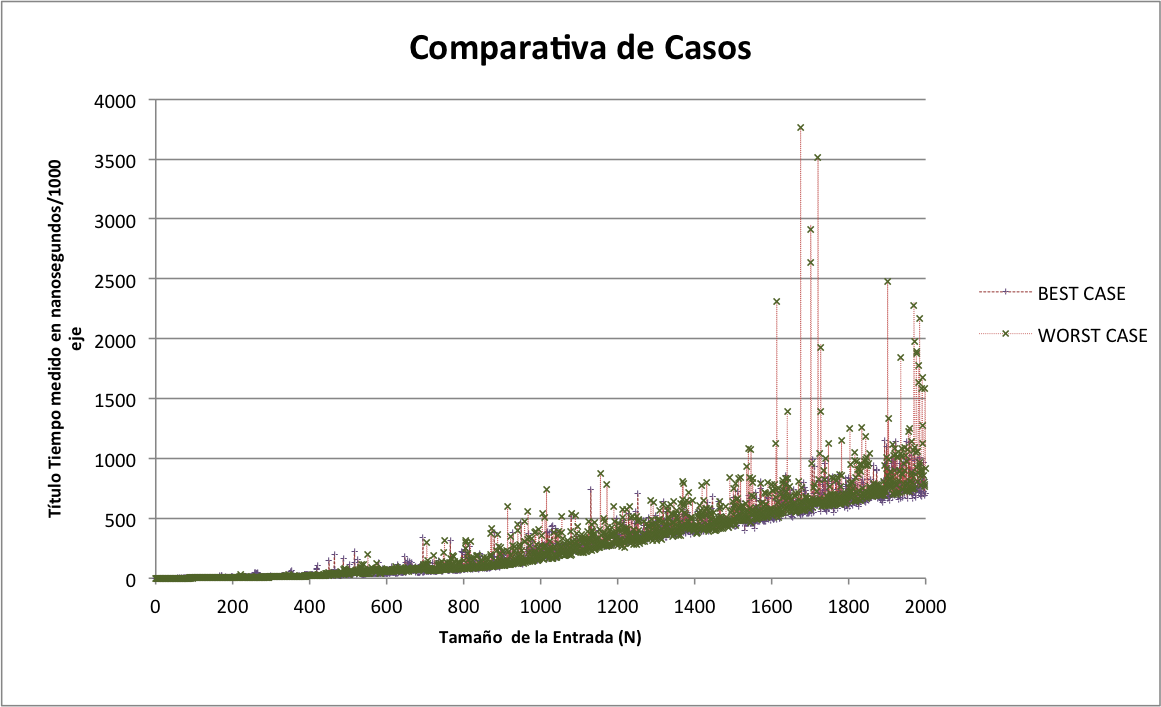
\includegraphics[width=140mm]{ej1-comp-tp2.png}
\centering
\caption{Comparaci\'on de matrices sin portales y completas.}
\label{overflow3}
\end{figure}

Efectivamente sucede lo que sospechabamos en la seccion anterior: En la primera figura vemos como el mejor y el peor caso se comportan asintoticamente de la misma manera ya que no importa qu\'e portales tengamos, la parte superior de la matriz se completa siempre.\\ 

\begin{figure}[h!]
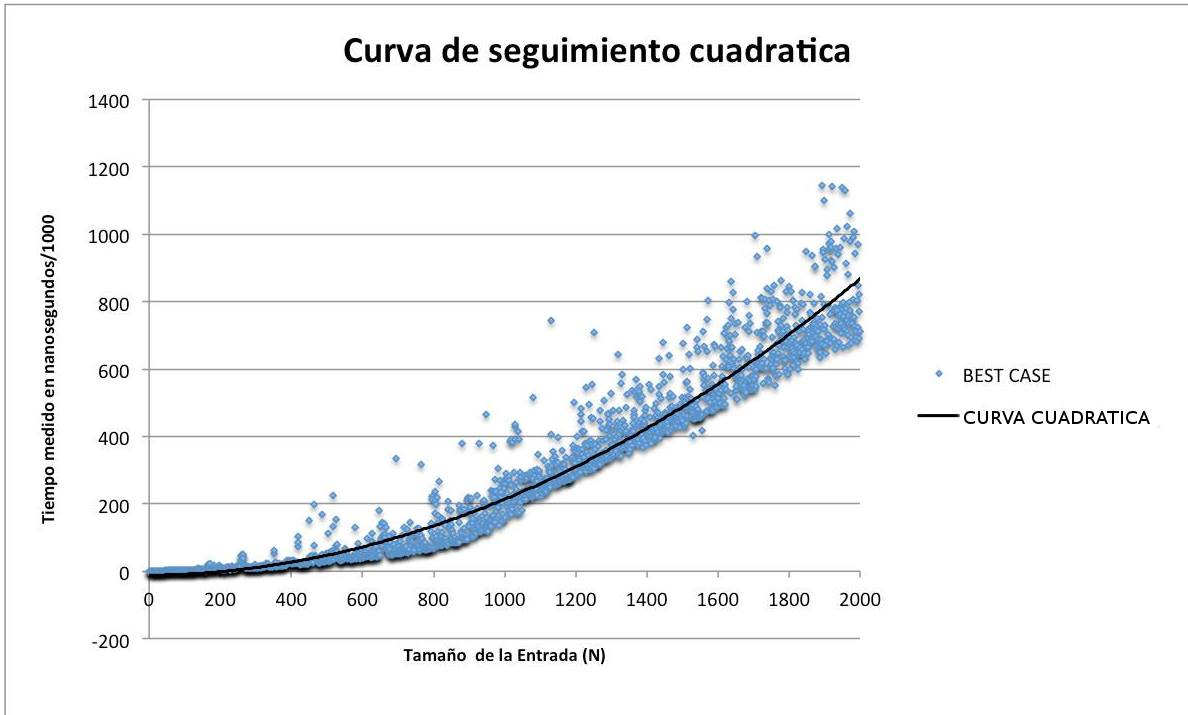
\includegraphics[width=140mm]{ej1-comp2-tp2.png}
\centering
\caption{Comparaci\'on de matrices sin portales y funcion cuadratica.}
\label{overflow3}
\end{figure}

En este segundo gr\'afico podemos ver que el comportamiento del algoritmo se puede aproximar con una curva cuadr\'atica multiplicada por una constante baja. Esto sucede porque como hab\'iamos mencionado anteriormente, nunca se recorre la matriz entera.

\pagebreak
